\subsection{Space-point reconstruction}
\label{Sect:SciFiSpcPnt}

This section describes the space-point reconstruction, the algebra by which the cluster positions are translated in to tracker coordinates and, to some extent, the algorithm.

\subsubsection{Selection of clusters that form the space-point}

For each particle event, the clusters found within each doublet layer are ordered by fibre-channel number. Taking each station in turn, an attempt is made to generate a space point using all possible combinations of clusters. The three clusters, one each from views $u$, $v$ and $w$, that make up a space point satisfy:

\begin{equation}
 n^u + n^v + n^w = n^u_0 + n^v_0 + n^w_0 \, ;
\end{equation}
where $n^u$, $n^v$ and $n^w$ are the fibre numbers of the clusters in the $u$, $v$ and $w$ views respectively and $n^u_0$, $n^v_0$ and $n^w_0$ are the respective central-fibre numbers (see Appendix~\ref{App:SciFiKuno}).

A triplet space point is selected if:

\begin{equation}
  | (n^u + n^v + n^w) - (n^u_0 + n^v_0 + n^w_0) | < K \, .
\end{equation}
Once all triplet space-points have been found, doublet space-points are created from pairs of clusters from different views.

\subsubsection{Crossing-position calculation}

\paragraph{Doublet space-points}
\label{Para:DoubletSpacepoint}

The position of the doublet space-point in station coordinates, ${\bf r}_s$, is given by:

\begin{eqnarray}
  {\bf r}_s & = & \left( 
                      \begin{array}{c}
                        x_s \\ y_s
                      \end{array}
                     \right)                                  \\
               & = & \underline{\underline{R}}_{SD1} {\bf m}_1 
                                              \label{Eq:DSP1} \\
               & = & \underline{\underline{R}}_{SD2} {\bf m}_2 
                                              \label{Eq:DSP2} \, ;
\end{eqnarray}
where the measurement vector corresponding to the $i^{\rm th}$ cluster: 

\begin{equation}
  {\bf m}_i = \left( 
               \begin{array}{c}
                 \alpha_i \\ \beta_i
               \end{array}
              \right) \, ;
\end{equation}
and the rotation matrix $\underline{\underline{R}}_{SDi}$ are defined in section~\ref{SubSect:SciFiHtsClstrs}. The simultaneous equations~\ref{Eq:DSP1} and \ref{Eq:DSP2} contain two unknowns, $\beta_1$ and $\beta_2$. Equations~\ref{Eq:DSP1} and \ref{Eq:DSP2} may be rewritten:

\begin{equation}
  {\bf m}_1 = \underline{\underline{R}}_{SD1}^{-1}
              \underline{\underline{R}}_{SD2} {\bf m}_2 \, .
\end{equation}
Defining:

\begin{eqnarray}
  \underline{\underline{S}} & = & \underline{\underline{R}}_{SD1}^{-1}
                                  \underline{\underline{R}}_{SD2}     \\
                            & = & \left( 
                                    \begin{array}{cc}
                                      s_{11} & s_{12} \\
                                      s_{21} & s_{22}
                                    \end{array}
                                   \right) \, ;
\end{eqnarray}
Equations \ref{Eq:DSP1} and \ref{Eq:DSP2} may be solved to yield:

\begin{eqnarray}
  \beta_2 & = & \frac{\alpha_1 - s_{11} \alpha_2}{s_{12}}     \\
  \beta_1 & = & s_{21} \alpha_2 + s_{22} \beta_2 \, .
\end{eqnarray}
The position of the space-point may now be obtained from equation~\ref{Eq:DSP1} or \ref{Eq:DSP2}.

\paragraph{Triplet space-points}

As shown in figure~\ref{Fig:SenseArea}, the fibres layout is of one of two types. In one case (right panel of figure~\ref{Fig:SenseArea}), the centre of the channels, one in each of the three views, cross intersect at a single point. In this case, the position of the crossing can be calculated as described in section~\ref{Para:DoubletSpacepoint}. When the area of overlap of the three channels forms a triangle (figure~\ref{Fig:SenseArea} left panel), the centre of area of overlap is given by:

\begin{eqnarray}
  \bar{x} & = & \frac{2}{3}c_p \, {\rm ; and}       \\
  \bar{y} & = & 0 \, .
\end{eqnarray}

\begin{figure}
  \begin{center}
    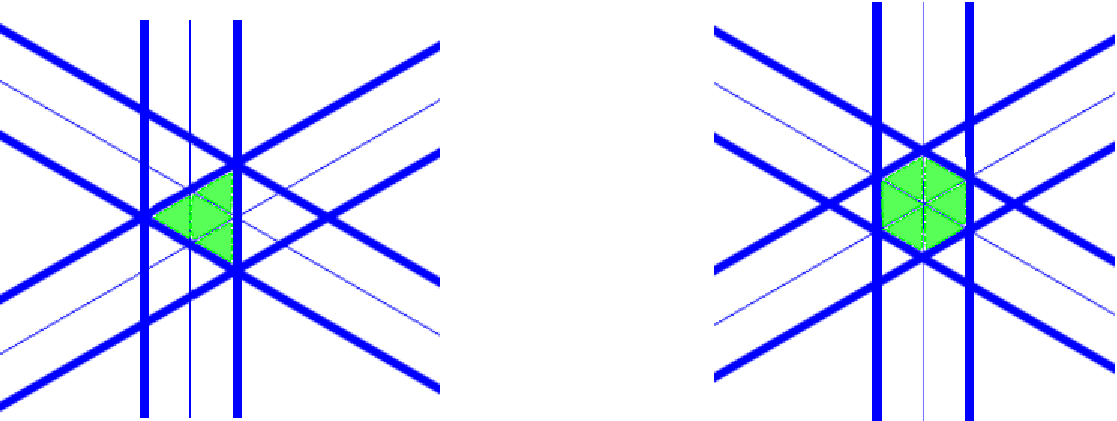
\includegraphics[width=0.7\linewidth]{detectors/tracker/04-Reconstruction/04-02-Space-points/Figures/SpacepointError.pdf}
  \end{center}
  \caption{Right panel: Fibre arrangement in station 5 of tracker 1. Left panel: Fibre arrangement in the rest of the stations. The shaded region shows the intersection of the three channels is triangle for every station other than station 5, where itwill be an hexagon.}
  \label{Fig:SenseArea}
\end{figure}
